\newcommand{\chapter}[2][]{
	\newcommand{\chapname}{#2}
	\begin{flushleft}
		\begin{minipage}[t]{\linewidth}
			
\includegraphics[height=1cm]{hdht-logo.png}
			\hspace{0pt}	
			\sffamily\bfseries\large Bài 6.
			\begin{flushleft}
				\LARGE\bfseries #1
			\end{flushleft}
		\end{minipage}
	\end{flushleft}
	\vspace{1cm}
	\normalfont\normalsize
}
\chapter[Thực hành: Đo tốc độ của vật chuyển động]{Thực hành: Đo tốc độ của vật chuyển động}

\subsection{Đo tốc độ trong phòng thực hành}
\subsubsection{Dùng cổng quang điện và đồng hồ đo thời gian hiện số}
Cổng quang điện là thiết bị gồm một cửa phát tia sáng, cửa đối diện thu tia sáng. Trên vật chuyển động có gắn một tấm chắn sáng, có tác dụng chắn chùm tia sáng truyền giữa hai cửa của cổng quang điện.
\begin{center}
	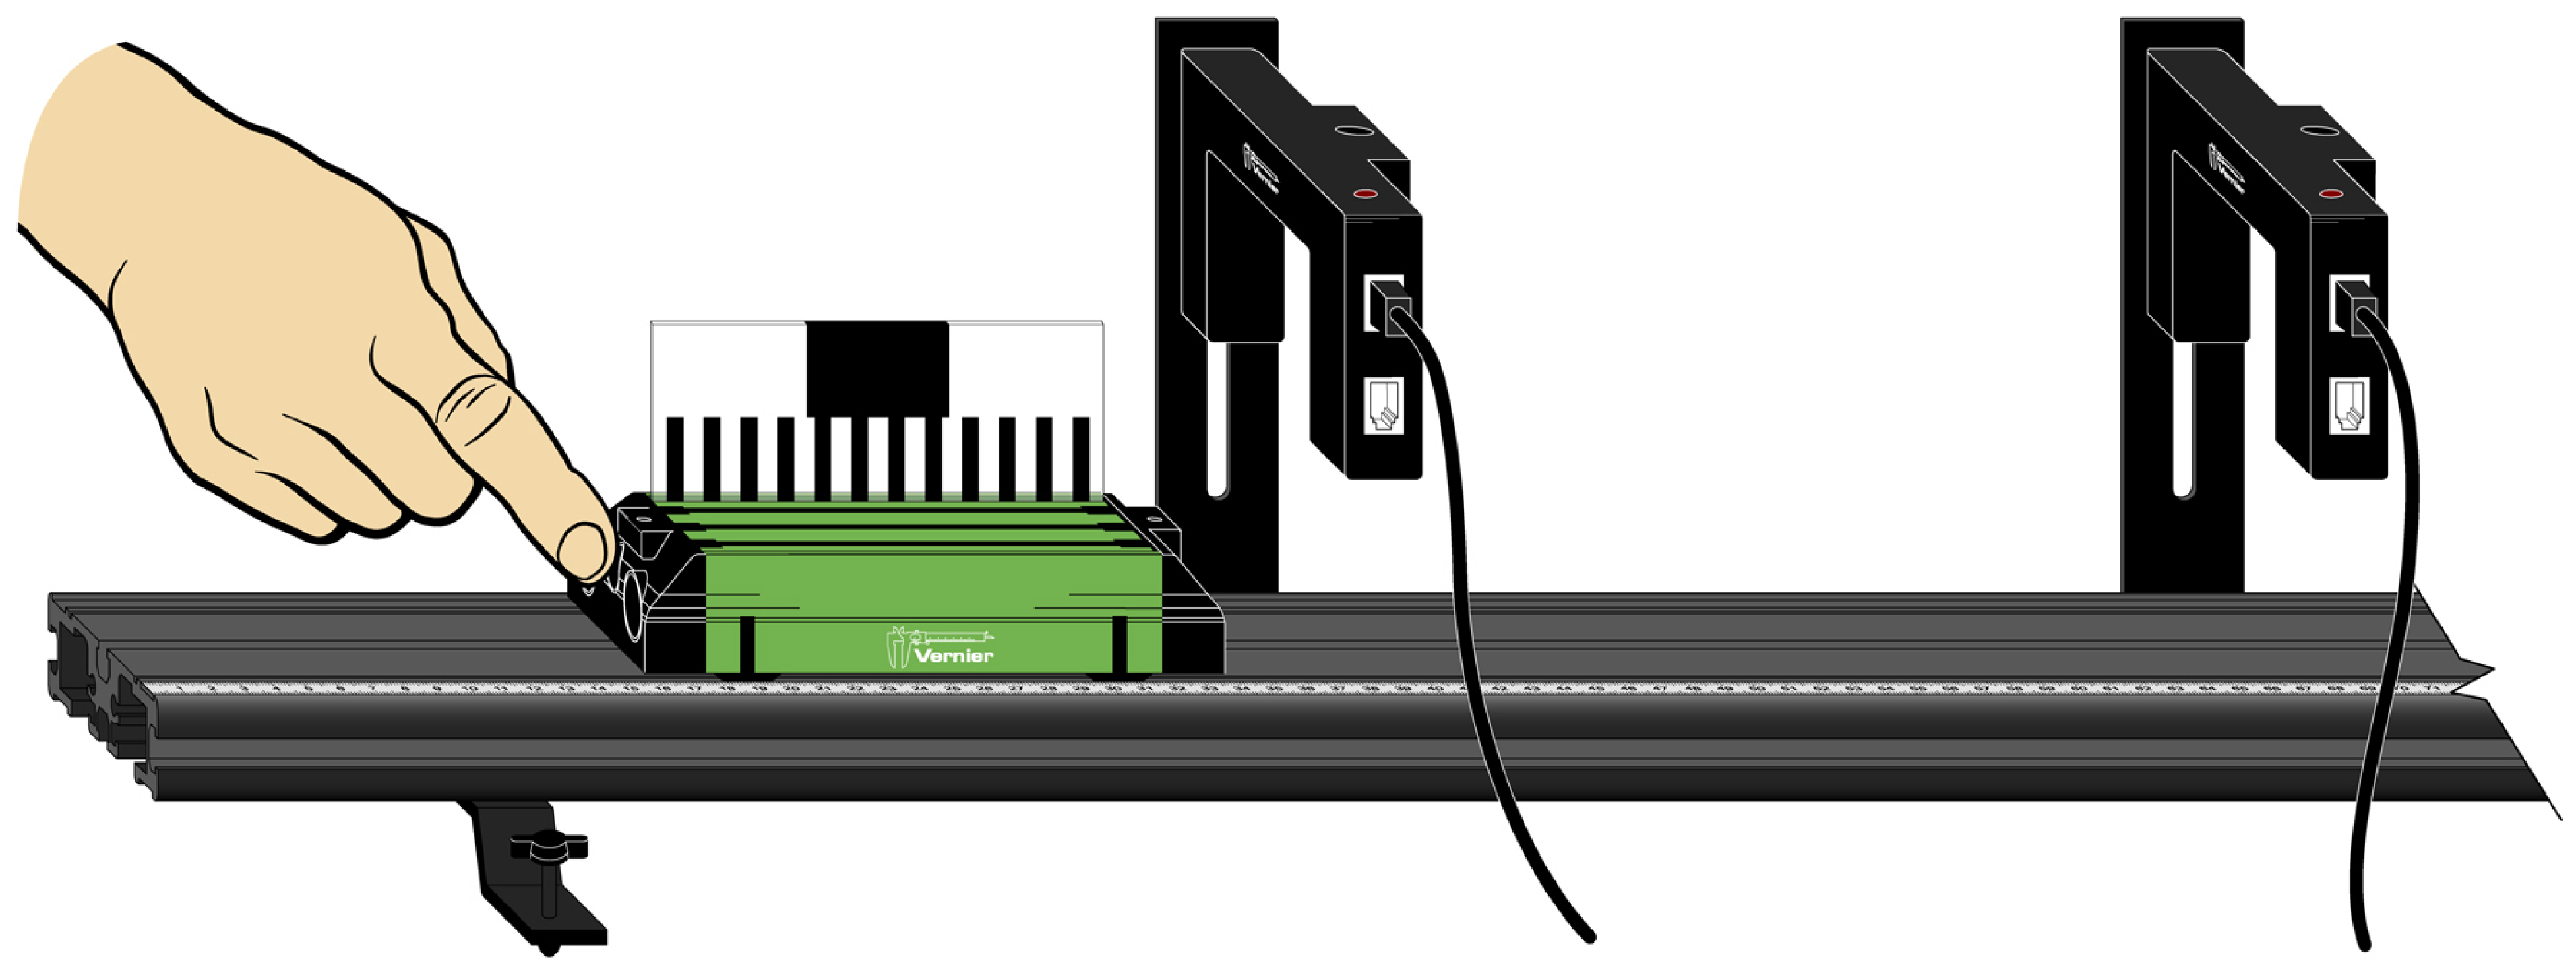
\includegraphics[width=0.5\textwidth]{../figs/G10-4-1}
\end{center}
%Có thể sử dụng kết hợp hai cổng quang điện để đo khoảng thời gian vật chuyển động trên quãng đường bằng khoảng cách giữa hai cổng, hoặc chỉ sử dụng một cổng quang điện để đo khoảng thời gian vật chuyển động được đoạn đường bằng kích thước của tấm chắn sáng.
Cổng quang điện được kết hợp với đồng hồ đo thời gian hiện số với nguyên tắc như sau:
\begin{itemize}
	\item Khi tấm chắn sáng bắt đầu chắn chùm tia sáng ở cổng quang điện thì đồng hồ bắt đầu đo thời gian.
	\item Ngay khi tấm chắn sáng không còn chắn chùm tia sáng nữa thì đồng hồ ngừng đo.
	\item Thời gian hiển thị trên đồng hồ là thời gian xe đi hết quãng đường bằng chiều rộng của tấm chắn sáng. %(hoặc bằng khoảng cách giữa hai cổng quang điện).
	\item Từ quãng đường và thời gian, ta rút ra được tốc độ chuyển động của vật: $v = \dfrac{s}{t}$.
\end{itemize}
\subsubsection{Dùng xe kĩ thuật số}
Đây là thiết bị có chức năng như đồng hồ đo tốc độ gắn trên các phương tiện như ô tô, xe máy,... Số liệu về tốc độ chuyển động của vật sẽ hiển thị trực tiếp trên màn hình của thiết bị.
\begin{center}
	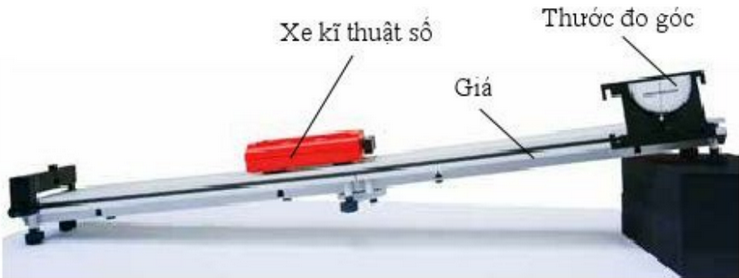
\includegraphics[width=0.5\textwidth]{../figs/G10-4-2}
\end{center}
\subsection{Ghi kết quả đo vào bảng số liệu và nhận xét}
\subsubsection{Lý thuyết nền tảng trước khi thực hành}
Trả lời được các câu hỏi sau:
\begin{itemize}
	\item Thế nào là chuyển động? Thế nào là chuyển động thẳng đều?
	\item Phân biệt quãng đường, độ dịch chuyển (độ dời), tốc độ, vận tốc, tốc độ trung bình.
	\item Các loại sai số trong phép đo các đại lượng vật lý, cách viết kết quả đo, cách nhận xét kết quả đo.
	\item Các quy tắc an toàn trong phòng thực hành vật lý.
\end{itemize}
\subsubsection{Cách trình bày kết quả đo}

\begin{center}
	\vspace{5pt}
	\begin{tabular}{|c|c|c|c|c|}
		\hline
		\textbf{Lần đo $n$}& Độ dịch chuyển & Sai số & Thời gian & Sai số\\
		&(m)&(m)&(s)&(s)\\
		\hline
		1&&&&\\
		\hline
		2&&&&\\
		\hline
		3&&&&\\
		\hline
		4&&&&\\
		\hline
		5&&&&\\
		\hline
		\textbf{Giá trị trung bình }&&&&\\
		\hline
	\end{tabular}
\end{center}
trong đó:
\begin{itemize}
	\item Giá trị trung bình $\bar{s} = \dfrac{s_1 + s_2 + s_3 + \ldots + s_n}{n}$;
	\item Sai số $\Delta s_n = |\bar{s} - s_n|$. 
\end{itemize}

Kết quả đo được viết dưới dạng  $$s=\bar{s} \pm (\Delta s)_\text{max}.$$
Cách tính và viết kết quả đo này được áp dụng cho thời gian và vận tốc.

%Ngoài ra, ta còn phải viết đúng số chữ số có nghĩa trong kết quả đo và tuân thủ quy tắc làm tròn số:
%\begin{itemize}
%	\item Chữ số có nghĩa là những số khác 0, hoặc là số 0 ở cuối mỗi số và ở bên phải dấu thập phân, hoặc là số 0 nhưng đứng ở giữa những số khác 0, và những số biểu thị lũy thừa, căn thức.
%	\item Với kết quả cộng và trừ, kết quả cuối cùng có số thập phân bằng đúng số thập phân của thành phần kém chính xác nhất.
%	\item Với kết quả nhân và chia, kết quả cuối cùng có số chữ số có nghĩa bằng đúng số chữ số có nghĩa của thành phần có ít số chữ số có nghĩa nhất. Quy tắc này áp dụng tương tự với lũy thừa và căn thức.
%	\item Trong các phép tính, hạn chế làm tròn ở các bước trung gian.
%\end{itemize}
% Hưng's comment: cách giải thích chữ số có nghĩa như trên chưa rõ, nếu cần phải tách thành mục riêng, có ví dụ rõ ràng. Trong sách giáo khoa Vật lý 10 hiện giờ (chương trình cũ) phần này viết bị sai và chưa đầy đủ các trường hợp nên dễ gây nhầm lẫn cho học sinh. Tạm thời sẽ bỏ phần này. 
\subsection{Biểu diễn kết quả đo lên phần mềm máy vi tính và cách sử dụng Excel để biểu thị kết quả đo}
Khi biểu diễn kết quả đo của một vật chuyển động thẳng đều lên phần mềm máy vi tính, ta có đồ thị như sau:
\begin{center}
	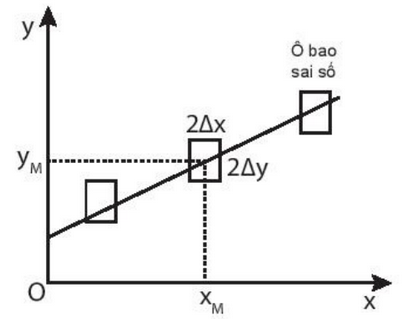
\includegraphics[scale=0.8]{../figs/G10-4-3.png}
\end{center}
Trong đó, $x$ và $y$ lần lượt biểu thị cho thời gian (s) và quãng đường dịch chuyển (m).

Một trong những phần mềm đơn giản và phổ biến để biểu diễn đồ thị kết quả đo là phần mềm Microsoft Excel:
\begin{itemize}
	\item Mở file Excel có chứa dữ liệu thu thập được từ thực hành, hoặc tạo mới file Excel và ghi dữ liệu thu thập được;
	\item Tô chọn vùng dữ liệu sẽ xuất hiện trong đồ thị;
	\item Chọn thẻ Insert $\rightarrow$ Chọn mục Charts;
		\begin{center}
			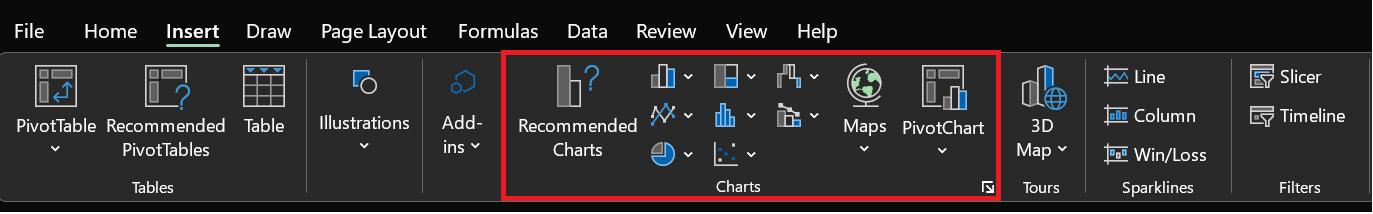
\includegraphics[width=0.85\textwidth]{../figs/G10-4-4}
		\end{center}
	\item Chọn kiểu đồ thị mong muốn;
		\begin{center}
			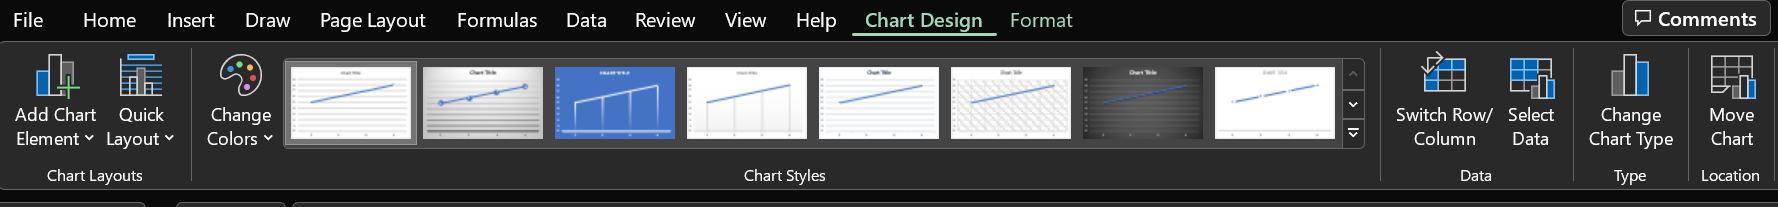
\includegraphics[width=0.85\textwidth]{../figs/G10-4-5}
		\end{center}
	\item Điều chỉnh các thông tin trong đồ thị theo ý muốn.
		\begin{center}
		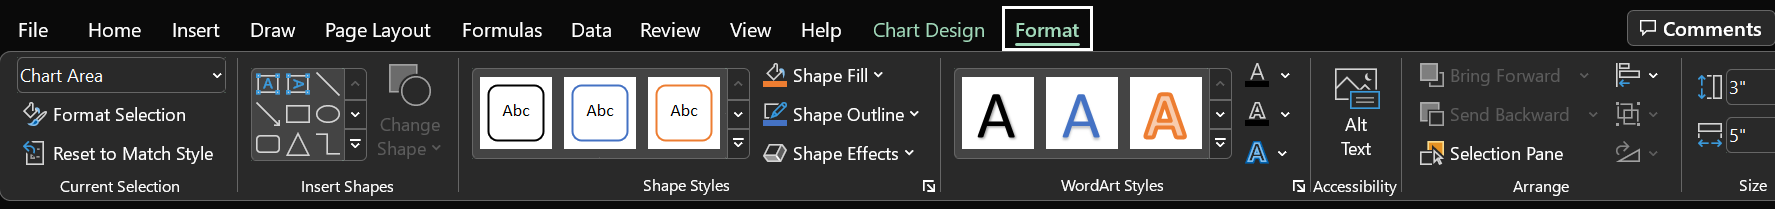
\includegraphics[width=0.85\textwidth]{../figs/G10-4-6}
		\end{center}
\end{itemize}